\documentclass[10pt, conference, compsocconf]{IEEEtran}
\usepackage[T1]{fontenc}
\usepackage[utf8]{inputenc}
\usepackage[brazilian]{babel}
\usepackage{verbatim}
\usepackage{scalefnt}
\usepackage{xcolor}
\usepackage{ulem}
\usepackage{type1cm}
\usepackage{url}
\usepackage{subfigure}
\usepackage{courier}
\newcommand{\TODO}[1]{{\color{red}\textbf{\uwave{#1}}}}

\usepackage[pdftex]{graphicx}
\DeclareGraphicsExtensions{.png}

\title{Práticas de colaboração no desenvolvimento de Software com o Governo: impactos na aprendizagem de alunos de graduação}

\author{
	\IEEEauthorblockN{Camila Ferreira$^1$, Aline Gonçalves$^1$, Marisa Santos$^2$, Paulo Meirelles$^1$, Hilmer Neri$^1$}
	\IEEEauthorblockA{
		$^1$Faculdade UnB Gama -- Universidade de Brasília (UnB), Brasil\\
		$^2$Ministério do Planejamento, Orçamento e Gestão (MP), Brasil\\
		\{camilaferreira251,alinegsantoss\}@gmail.com, marisa.santos@planejamento.gov.br, \{paulormm,hilmer\}@unb.br
	}

}

%-------------------------------------------------------------------------------
\begin{document}
\normalem
\def\UrlFont{\tt\footnotesize}
\maketitle

\begin{abstract}
O Portal do Software Público Brasileiro (SPB), na prática, é um sistema web
que se consolidou como um ambiente de compartilhamento
de softwares. O projeto de evolução deste portal está sendo desenvolvido pela 
Universidade de Brasília e conta com integrantes de diversos perfis e níveis de formação. O 
projeto utiliza algumas práticas de métodos ágeis em sua metodologia de desenvolvimento. O 
objetivo deste artigo é relatar a experiência no desenvolvimento, ao lado do Ministério de Planejamento, bem como mostrar o quanto o projeto tem contribuído para a formação dos seus 
integrantes.

\end{abstract}
\vspace{1\baselineskip}

\begin{keywords}
Engenharia de Sofware, Software Livre, Software Público, Evolução de Software
\end{keywords}





\IEEEpeerreviewmaketitle

%-------------------------------------------------------------------------------

\section{Introdução}
\label{sec:introducao}

O governo federal brasileiro vem nos últimos anos buscando melhorias nos
seus processos de desenvolvimento e adoção de software.
%
Desde 2003, a recomendação da adoção de software livre passou a ser uma política
incentivada na esfera federal, inicialmente com a criação do
Guia Livre\footnote{governoeletronico.gov.br/acoes-e-projetos/guia-livre}.
%
Hoje, tal iniciativa é coordenada pelo Comitê Técnico de Implementação de
Software Livre do Governo Federal\footnote{softwarelivre.gov.br}.


No contexto da promoção do software livre no governo federal, a
Secretaria de Logística e Tecnologia da Informação (SLTI) do Ministério do
Planejamento, Orçamento e Gestão (MP) inaugurou em 2007, o Portal do Software
Público Brasileiro (SPB), que, na prática, é um sistema web que se consolidou como
um ambiente de compartilhamento de projetos de software no governo.
%
Por exemplo, a Instrução Normativa
04/2012\footnote{governoeletronico.gov.br/biblioteca/arquivos/instrucao-normativa-no-04-de-12-de-novembro-de-2010}
indica que os gestores devem consultar as soluções existentes no Portal do SPB
antes de realizar uma contratação de software.
%
Hoje, com o portal do SPB tem cerca de 69 comunidades de
desenvolvimento e mais de 200.000 usuários cadastrados.

Entretanto, a evolução do SPB foi comprometida, desde 2009, quando a plataforma
do SPB não acompanhou a evolução do seu arcabouço base,
o \emph{OpenACS}\footnote{openacs.org}.
%
Com isso, não tendo versões lançadas a partir daquele ano.

Nesse contexto, um dos passos para a concretização de uma nova plataforma para o
SPB é a integração com novas tecnologias, desde uma plataforma colaborativa até sistemas
de controle de versão e de monitoramento da qualidade do código-fonte.
%
Para concretizar a evolução do SPB, a Universidade de Brasília está coordenando
tal processo, através de uma equipe heterogêne de alunos, professores e
profissionais, que estão aplicando práticas colaborativas de desenvolvimento
de software e gestão de projeto que impactam no projeto em si e, em especial,
na aprendizagem dos envolvidos.





\section{Arquitetura e tecnologias propostas}
\label{sec:arquitetura}

O sistema que irá atender a evolução e reformulação do Portal do Software Público Brasileiro é composto por diversos módulos, os quais irão comunicar-se entre si de forma organizada e integrada para suprir as necessidades do projeto.
%

\begin{figure}[htpb]
  \begin{center}
    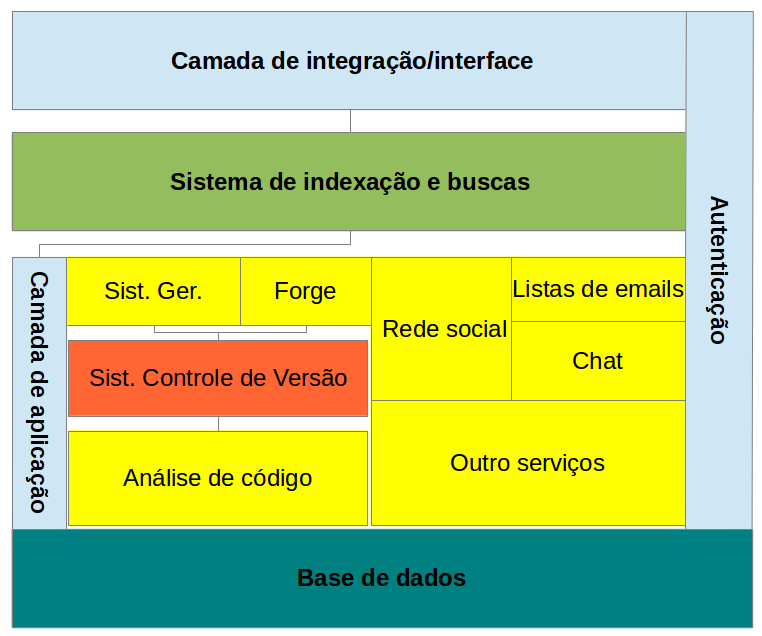
\includegraphics[width=.37\textwidth]{images/visao_arq.png}
  \end{center}
  \caption{Proposta de arquitetura do Novo Portal do Software Público}
  \label{fig:core_concurrent}
\end{figure}

No início do projeto realizamos estudos de possíveis ferramentas que pudessem ser utilizadas para atender as necessidades do projeto, chegando então na lista apresentada abaixo.
Na análise realizada chegamos ao entendimento que utilizar elementos já oferecidos por softwares livres existentes seria o ideal, pois eles já atendem às nossas necessidades, evitando o retrabalho e customizando os elementos necessários.   

As ferramentas que serão utilizadas para suprir essas necessidades serão:


\begin{itemize}
\scalefont{0.95}

\item Para lista de e-mail estamos utilizando o Mailman na versão 2, que é um software gratuito para gerenciamento de discussão eletrônica de e-mail e listas {\it e- newsletter};

\item Para Chat estamos utilizando Punjab BOSH (XMPP), que é uma interface HTTP cliente jabber. É um gerenciador de conexão BOSH que permite conexões de clientes persistentes para um servidor XMPP (protocolo de comunicação para mensagens orientadas a {\it middleware} baseado em XML);

\item Para Plataforma de Buscas estamos utilizando Apache Solr, que é uma plataforma de busca open source da Apache Lucene escrita em Java;

\item Para rede social estamos utilizando o Noosfero que é uma plataforma web livre para criação de redes sociais com blog, e-Portifólios, CMS, RSS, discussão temática, agenda de eventos, galeria de imagens, chat, entre outros. Ele foi desenvolvido pela Cooperativa de Tecnologias Livres – Colivre 3 em 2007, sob a licença AGPL v.3, com a proposta de permitir ao usuário criar sua própria rede social personalizada, livre e autônoma;

\item Para Forge para SVN estamos utilizando o Trac, que é uma ferramenta open source para controle de mudanças em projetos de desenvolvimento;

\item Para sistemas de controle de versão estamos utilizando SVN e Git, que são ferramentas open-source para controle de mudanças em projetos de desenvolvimento;

\item Para Forge para Git estamos utilizando o GitLab, que é um software livre de colaboração de código online que utiliza a ferramenta de gerência de código fonte Git;

\item Para sistema de gerenciamento estamos utilizando o Redmine, que é uma aplicação web de gerenciamento de projetos que disponibiliza diversas ferramentas para auxiliar a gestão e manutenção de um projeto;

\item Para suporte a Single Sign On estamos utilizando o Mozilla Persona, que foi desenvolvido pela Mozilla e permite o suporte a {\it single sign on};

\item Para Sistema de Integração contínua estamos utilizando o Jenkins, que é uma aplicação web de integração contínua de construção de projetos.
\scalefont{1}
\end{itemize}


Para integrar todas estas ferramentas estamos utilizando o Colab, que é uma plataforma de integração de ferramentas. Nele, são também integradas as interfaces das ferramentas para que, ao navegar, o usuário tenha a sensação de estar navegando em uma única ferramenta.



\section{Metodologia}
\label{sec:metodologia}

\subsection{Escolha da equipe}
\label{sec:equipe}

A equipe é formada, majoritariamente, por alunos de graduação do curso de Engenharia de Software da Universidade de Brasília, conta ainda com dois ex-alunos formados, alunos de mestrado, que trabalham exclusivamente com o design, e professores orientadores. 
	
	Devido a esta formação, a equipe não consegue estar sempre trabalhando fisicamente junta, pois cada membro da equipe possui horários particulares de aula e, com isso, o horário dedicado a contribuição do projeto pelos mesmos depende do horário dessas aulas. Dessa forma, não conseguimos utilizar integralmente as práticas das metodologias ágeis.
	
	A equipe do projeto está dividida em duas equipes: equipe Noosfero e equipe Colab, a qual também atua na integração com outras ferramentas. A equipe do Noosfero está desenvolvendo um plugin com novas funcionalidades para o Portal do Software Público. A equipe do Colab está, no momento, trabalhando com configurações das ferramentas, pois está sendo realizada a integração do Redmine e do Gitlab com o Colab, o que exige maiores esforços de infra-estrutura.
	
	Para manter o controle das atividades do projeto e evitar os ruídos de comunicação temos uma lista de e-mail com todos os integrantes do projeto, onde foi criado o hábito de enviarmos um e-mail ao final do dia com as atividades que desenvolvemos, e a ferramenta de gerenciamento Redmine, onde são escritas as histórias de usuários, as histórias técnicas e suas respectivas tarefas. Realizamos ainda um stand-up em todos os dias de trabalho,em que todos estão ou no laboratório ou presente virtualmente para alinharmos a situação das equipes. 
	
	Estamos trabalhando em sprints/ciclos de duas semanas, em média, e releases de quatro meses, sendo que o projeto tem duração programada de três anos, sendo ao total sete releases e cinquenta e oito sprints.


\subsection{Métodos de desenvolvimento e Gestão do Projeto}
\label{sec:metodo-gestao}

A Engenharia de Software tem evoluído suas práticas e metodologias em busca de padrões que regem o desenvolvimento de software de qualidade dentro dos escopos, custos e prazos desejados. 
%
Dada a oportunidade de adoção de métodos ágeis no desenvolvimento do presente trabalho, a 
metodologia utilizada é baseada em uma combinação das metodologias Scrum e Extreme Programming. Destacam que XP e Scrum complementam um ao outro bem, com o XP provendo suporte para aspectos mais técnicos enquanto o Scrum provê práticas e técnicas para gerenciamento, planejamento e acompanhamento. Assim,com base nas experiências destacadas em~\cite{schwaber2001} e~\cite{fitzgerald2006}, na motivação de adoção de métodos ágeis no desenvolvimento de software moderno, serão apresentadas os métodos XP e Scrum, suas principais características e práticas que serão utilizadas no desenvolvimento do presente projeto.

%TODO ...



\section{Relato de Experiência}
\label{sec:estudo}

Foi aplicado um questionário na equipe de desenvolvimento do Novo Portal do Software Público, onde os mesmos poderiam expressar o quanto estão aprendendo com o projeto e o quanto o projeto está ajudando na sua formação.

O questioário foi respondido por 17 integrantes do projeto que têm entre 20 e 26 anos, os quais então entre o 5º e o 10º semestre do curso de Engenharia de Software.

A primeira questão pretendia averiguar o nível de conhecimento dos entrevistados, em uma escala de 1 a 5, em relação às ferramentas que estão sendo utilizadas no projeto. Como resultados tivemos que 63\% responderam nível 3, 19\% responderam nível 2 e 19\% responderam nível 4.

A segunda questão pretendia averiguar o quanto o projeto está contribuindo para a formação do entrevistado. Em uma escala de 0 a 5, 69\% dos entrevistados responderam "5 -Contribui muito, mais que determinadas disciplinas", 19\% dos entrevistados responderam "4 - Contribui, no mesmo nível de muitas disciplinas" e 13\% dos entrevistados responderam "3 - Contribui, da mesma forma que um estágio convencional".

\begin{figure}[htpb]
  \begin{center}
    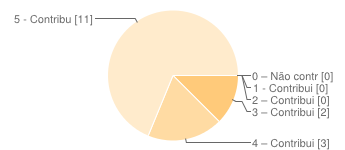
\includegraphics[width=.37\textwidth]{images/chart1.png}
  \end{center}
  \caption{Respostas do nível de contribuição do projeto na sua formação}
  \label{fig:core_concurrent}
\end{figure} 

A terceira questão está relacionada, também em uma escala de 0 a 5, a quanto o projeto atrapalha a sua performance nas disciplinas da graduação. Como resultados, 19\% dos entrevistados responderam "3 - Atrapalha minha graduação da mesma forma que um estágio", 50\% dos entrevistados responderam "2 - Atrapalha moderadamente", 19\% dos entrevistados responderam "1 - Atrapalha pouco, menos que um estágio" e 13\% dos entrevistados responderam "0  Não atrapalha em nada na minha graduação".

\begin{figure}[htpb]
  \begin{center}
    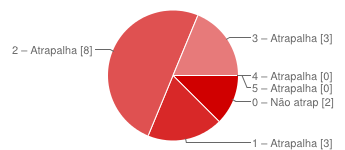
\includegraphics[width=.37\textwidth]{images/chart2.png}
  \end{center}
  \caption{Respostas do nível de performance nas disciplinas de graduação}
  \label{fig:core_concurrent}
\end{figure} 

A quarta questão averigua o quanto, em uma escala de 0 a 5, os conhecimentos adiquiridos durante a execução do projeto ajudam os entrevistados nas disciplinas da graduação. Como resultados, 7\% dos entrevistados responderam "5 - Ajuda muito, sempre utilizo os conhecimentos adiquiridos nas disciplinas da graduação	", 47\% respondeu "4  Ajuda muito, utilizo os conhecimentos com frequência nas disciplinas da graduação", 27\% respondeu "3 - Ajuda, utilizo os conhecimentos nas disciplinas da graduação" 13\% respondeu "2 - Ajuda moderadamente, as vezes utilizo os conhecimentos adquiridos no projeto" e 7\% respondeu "1 – Ajuda um pouco, utilizo pouco os conhecimentos do projeto".

\begin{figure}[htpb]
  \begin{center}
    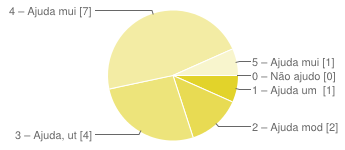
\includegraphics[width=.37\textwidth]{images/chart3.png}
  \end{center}
  \caption{Respostas do nível de conhecimento adquirido}
  \label{fig:core_concurrent}
\end{figure} 

E a quinta questão perguntou o quanto, em uma escala de 0 a 5, o entrevistado acredita que o projeto do Novo SPB vai contribuir em experiência para o mercado de trabalho. Como resultados, 38\% responderam "5  O projeto me tornará experiente para o mercado de trabalho", 38\% responderam "4 - O projeto me dará muita experiência para o mercado de trabalho" e 25\% responderam "3 - O projeto me dará uma boa experiência para o mercado de trabalho".

\begin{figure}[htpb]
  \begin{center}
    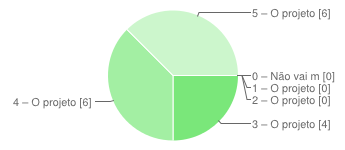
\includegraphics[width=.37\textwidth]{images/chart4.png}
  \end{center}
  \caption{Respostas do nível de experiência para o mercado de trabalho}
  \label{fig:core_concurrent}
\end{figure} 

\subsection{Discussão dos resultados}

Já era esperado o resultado da questão relacionada ao nível de experiência da equipe com as ferramentas a serem utilizadas pois, era sabido que por serem alunos de graduação já poderiam ter tido alguma experiência com as ferramentas nas disciplinas sem chegar a ser usuário avançado ou desenvolvedores experientes nas mesmas, mas teriam algum conhecimento que auxiliaria na execução das atividades.

O projeto tem como objetivo auxiliar na formação dos alunos e por isso foi questionada a opinião dos alunos à respeito da contribuição trazida pelo projeto para sua formação, obtivemos respostas positivas para essa pergunta pois o projeto proporciona um ambiente de aprendizado e conhecimento de novas tecnologias e metodologias de desenvolvimento além de adiantar problemáticas que ainda serão vistas nas disciplinas da graduação.

Sabendo que o projeto retira do aluno horas semanais que poderiam estar destinadas ao estudo para as disciplinas da graduação, trouxemos a questão de quanto o projeto atrapalha no desempenho das disciplinas da graduação. As respostas foram mais variadas, alguns responderam que não atrapalha em nada na graduação, outros que atrapalham menos ou da mesma forma que um estágio e a maioria respondeu que atrapalha moderadamente, ou seja, o projeto está atrapalhado na graduação mas é compensado pelo conhecimento adquirido já que nenhum entrevistado respondeu que está se sentindo prejudicado por causa do projeto.

O projeto têm auxiliado nas disciplinas da graduação, segundo os entrevistados, como já mencionado, sendo assim o projeto adianta para os integrantes alguns assuntos que ainda seriam vistos nas disciplinas de graduação, diminuindo a curva de aprendizados dessas disciplinas durante a graduação.

Uma preparação para o mercado de trabalho é importante e segundo os entrevistados o projeto está trazendo uma boa experiência profissional para os seus integrantes. O contexto de um projeto real com prazos e necessidades específicas em diferentes áreas da engenharia de software devem ter sidos pensadas pelos entrevistados para a resposta desta questão. 

O projeto também tem beneficiado o aprendizado dos alunos em temas relacionados a Administração Pública pois o Portal do SPB é um sistema web que também visa beneficiar aos órgãos das esferas federal, estadual e municipal. Essa relação com o governo auxilia tanto no crescimento profissional, uma vez que estabelece um contato com usuários de governo, como uma visão sobre negócios que envolvem toda a Administração Pública.

\section{Conclusão}
\label{sec:conclusao}

Neste projeto são utilizadas diversas ferramentas que não têm sua linguagem de programação em comum e sobretudo são relativamente novas no mercado e mesmo com esses impecilhos podemos afirmar, a partir do relato de experiência, que os alunos não tinham experiêcia nas ferramentas a serem utilizadas no projeto mas esta aparente dificuldade não impediu os alunos de contribuir com o projeto

Foi possível concluir também que o projeto está contribuindo com a construção da formação dos alunos, pois coloca em prática algumas situações antes vistas apenas na teoria dentro da sala de aula. 
%
O desempenho dos alunos nas disciplinas da graduação também é ajudado pelo projeto,devido ao conhecimento prévio adquirido não somente de práticas ágeis mas também de novas linguagens de programação. 
%
Ficou conhecido também que tempo gasto trabalhando no projeto atrapalha moderadamente o desempenho na graduação dos integrantes do projeto, mas o esforço será recompensado com uma boa experiência para o mercado de trabalho.

De maneira geral o projeto tem ajudado os seus integrantes a aprender a lidar com dificuldades encontradas no desenvolvimento de software, está trazendo conhecimento técnico e gerencial para os membros da equipe além de auxiliar nas relações interpessoais.

%-------------------------------------------------------------------------------

\bibliographystyle{IEEEtran}
\bibliography{myReferences}
\end{document}
